%----------------------------------------------------------------------
\section*{Sobre el autor y el cuaderno de proyectos}
%----------------------------------------------------------------------

\begin{wrapfigure}{r}{0.4\linewidth}
	\centering
	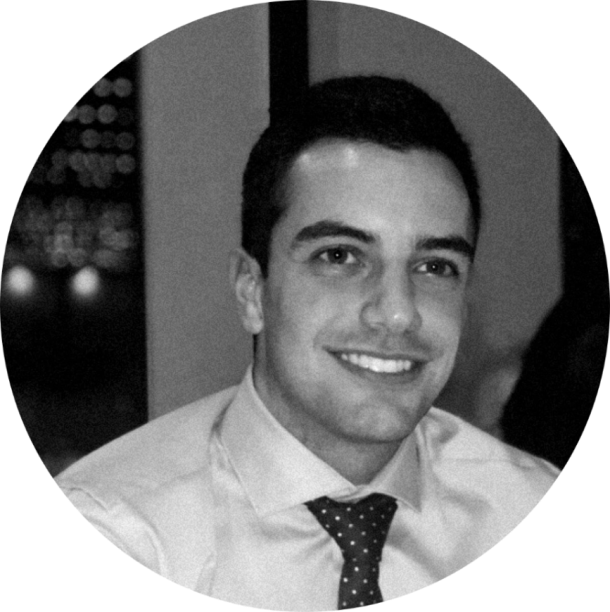
\includegraphics[width=0.4\textwidth]{me.png}
	\caption*{El autor}
	\label{labelformat=empty}
\end{wrapfigure}

Desde pequeño he sentido una gran curiosidad por saber cómo funcionan los objetos y máquinas que me rodean: radios, televisores, ordenadores... Pero si hay algo que me apasione son los aviones y el espacio. Ambos constituyen mis temas principales a la hora de desarrollar nuevos proyectos. Así pues, la mayoría de artículos en el presente cuaderno están estrechamente relacionados con el ámbito de la ingeniería aeronáutica/aeroespacial.\\

A medida que han avanzado los años he aprendido diferentes habilidades que han dotado de mayor complejidad todos estos trabajos personales (si bien algunos de los proyectos son colectivos): conocimientos de electrónica, programación en diferentes lenguajes, edición de imagen y vídeo... \\

El siguiente documento muestra algunos de estos proyectos y tiene como objetivo poner de manifiesto las cualidades como ingeniero que yo mismo he ido aprendiendo y trabajando en mi persona. La teoría es fundamental, pero nada como la práctica para ponerla de manifiesto.\\

Si desea contactar con el autor, puede enviar un correo a la siguiente dirección:

\href{mailto:ingenierodeaviones@gmail.com}{ingenierodeaviones@gmail.com}.


